\chapter{Experiments}
\label{chap:Experiments}

\section{Training \& MTMC Hyperparameters}
In this subsection, we present the essential configurations and hyperparameters used during the training process for the Feature Extraction model and for the MTMC (Multi-Target Multi-Camera) tracking stage. These settings directly influence the model's performance and its ability to generalize across varying scenarios. All tests have been carried on n. 2 NVIDIA Tesla A4000 GPUs with 16GB of VRAM each.

A detailed description of the network setup, datasets used for the experiments, metrics, optimizer, scheduler, and data augmentation strategies is provided to offer insights into the experimental framework.

\subsection{Network setup}
As for the Feature Extraction model, a pre-trained ResNet-IBN-50 architecture has been used as backbone. The model weights are pre-trained on ImageNet and the model itself uses the BNNeck architecture, along with setting the last stride of the Convolutional Filter, in the last block, equal to 1, as previously explicited in \ref{subsubsec:Stride} and \ref{subsec:BNNeck}.

\subsection{Loss}
The loss function used for training the Feature Extraction model is the combination of the ID Loss and the Metric Loss, as described in \ref{subsec:LossFunctions}. The ID Loss, used to classify the input images into the correct class, follows a standard Cross Entropy with the label smoothing parameter $\beta = 0.20$. As for the Metric Loss, a standard Triplet Loss is used to minimize the distance between the anchor and the positive samples, and to maximize the distance between the anchor and the negative samples. Its margin parameter $\alpha$ is set to 0.3.
As for the MALW training loop, a standard parameter search was able to set $K = 2000$ as the most favorable value, hence every 2000 iterations the $\lambda_{ID}$ parameter (ID weight) gets updated following the standard deviation of the ID Loss itself, while the $\lambda_{Metric}$ parameter (Metric Loss weight) is simply set to 1.0.

\subsection{Dataloaders}
As for the Dataloaders, we follow what has been detailed in \ref{subsubsec:DataloaderSampling}, where \textit{Random Sampling} was chosen as the sampling strategy and the parameter $K$ and $P$ are set to 36 and 6, respectively, meaning that the number of identities per batch is set to 36, while the number of images per identity is set to 6. Furthermore, the number of workers has been set equal to 8.

\subsection{Datasets}
For the proposed methodology, multiple Datasets have been used between the Feature Extraction and MultiTrack Re-Identification tasks. The Datasets, which sum up to 7, differ in terms of the number of cameras, number of vehicles and number of images as can be seen from Table \ref{table:Datasets}.

\begin{table}[ht]
    \centering
    \caption{Dataset comparisons}
    \begin{tabular}{|C{0.80in}|C{1.00in}|C{0.80in}|C{0.80in}|C{0.85in}|}
    \hline
    \textbf{Dataset} & \textbf{Purpose} & \textbf{Images} & \textbf{Vehicles} & \textbf{Cameras} \\ \hline
    \hline
    VeRi-776 & Re-ID & 49,537 & 776 & 20 \\ \hline
    VehicleID & Re-ID & 221,763 & 26,267 & Multiple viewpoints \\ \hline
    VeRi-Wild & Re-ID & 416,314 & 40,671 & 174 \\ \hline
    VRU & Re-ID & 172,137 & 15,085 & Multiple viewpoints \\ \hline
    AICity & Re-ID/MultiTrack & - & 145 & 4 \\ \hline
    \end{tabular}
    \label{table:Datasets}
\end{table}

\subsubsection{VeRi-776}
\textbf{VeRi-776} \cite{Veri776_1, Veri776_2, Veri776_3} is a Vehicle Re-ID Dataset, widely accepted as a benchmark measure, specifically designed for real-world surveillance contexts to evaluate the proposed framework for Feature Extraction. With more than \textbf{50,000} images of \textbf{776} different vehicles captured during a continuous 24-hour period in an urban area of size 1.0 km$^2$, it is one of the largest-scale and most diverse datasets with detailed annotations, making it among the most complete publicly available datasets for Vehicle Re-ID research.

It is recorded with 20 non-overlapping cameras positioned in a view to simulate realistic traffic monitoring scenarios. This setup makes it well-scalable and retains challenges relevant to practical applications of Vehicle Re-Identification. Along with that, the following characteristic features make the dataset uniquely suitable for training and evaluating the feature extraction models in complex surveillance scenarios. Specifically:

\begin{itemize}
    \item \textit{Real-world Variants}: The images are captured in unconstrained surveillance scenes, and thus, exhibit a rich set of real-world challenges such as illuminations, various resolution scales and occlusions. The vehicles are recorded from 2 to 18 different views across multiple cameras, introducing significant intra-class variability while ensuring sufficient recurrence rates, which are essential for effective cross-camera vehicle re-identification.
    \item \textit{Attribute Annotations}: The images are fully annotated with various attributes like Vehicle ID, Camera ID, Color, and Type that make it possible to train a complex Neural Network model necessary in learning complex visual features discriminating between vehicles with very subtle appearance differences.
\end{itemize}

\subsubsection{VehicleID}
The \textbf{VehicleID} \cite{VehicleID} dataset consists of a large-scale Vehicle Re-Identification dataset captured during the daytime using multiple non-overlapping surveillance cameras deployed across a small city in China. Unlike some other datasets mainly designed to target fine-grained vehicle model classification, such as the CompCars dataset \cite{CompCars}, the VehicleID dataset aims to resolve real-world tasks of vehicle retrieval and re-identification. It emphasizes representing frequently observed vehicles with consideration to the imbalanced nature that exists in real-world distribution.

This dataset contains \textbf{221,763} images of \textbf{26,267} vehicles, at an average of \textit{8.44} images per vehicle. Each vehicle is captured under multiple viewpoints, mostly front or rear, although viewpoint information itself is not annotated.

Given the substantial scale of the Dataset, the authors further extracted three subsets from the Test Set, namely: Small, Medium, and Large towards a more efficient-aware scalable evaluation process. The various subsets are separated as follows:
\begin{itemize}
    \item \textit{Small}: 800 vehicles, 7,332 images.
    \item \textit{Medium}: 1,600 vehicles, 12,995 images.
    \item \textit{Large}: 2,400 vehicles, 20,038 images.
\end{itemize}

Besides vehicle identity labels, vehicle model annotations are provided, covering 250 of the most frequently observed vehicle models, such as "MINI Cooper," "Audi A6L," and "BMW 1 Series." The distribution of vehicle models is imbalanced, similar to reality; frequently observed models have more than 2,000 associated images, like "Buick Excelle" or "Volkswagen Lavida," whereas rarely observed models have only one or two images.

The VehicleID dataset outperforms others in scale, comprehensiveness of vehicle identities, and realism in the data distribution, therefore, being the ideal benchmark to evaluate a Re-ID method under realistic conditions in urban surveillance.

\subsubsection{VeRi-Wild}
The \textbf{VeRi-Wild} \cite{VeRi-Wild_1}, \cite{VeRi-Wild_2} dataset is a large-scale vehicle Re-Identification benchmark specifically designed to address the challenges of a real-world scenario. Collected from a CCTV surveillance system composed by 174 distributed cameras, the dataset spans a large urban area of over 200 km$^{2}$ and covers a time span of one month (30 days, 24 hours per day). With a complex and continuous collection containing these varied challenging situations, VeRi-Wild provides an indispensable asset in the evaluation and development of vehicle re-identification.

Raw data included 12M vehicle images, whereas after cleaning and one-month annotation of the data, the effort of 11 volunteers provided a dataset of \textbf{416,314} images of vehicles from \textbf{40,671} identities. In particular, the license plates were masked during annotation due to privacy reasons.

This dataset, as stated, has a number of important properties which reflect several real-world challenges in surveillance, like:
\begin{itemize}
    \item \textit{Unconstrained Capture Conditions}: The dataset is captured in an unconstrained scenario where all the variations in image quality, occlusions, and positions of the vehicles are naturally present. Vehicles can appear in more than 40 cameras, capturing varied conditions that pose significant challenges for the Re-ID algorithm.
    \item \textit{Complex Scenes of Urban Environments}: These 174 cameras are widely deployed across an urban district to capture vehicles against such complex backgrounds, resolutions, and perspectives. This introduces very large viewpoint variations and therefore becomes a very challenging task to identify vehicles across cameras.
    \item \textit{Severe Illumination and Weather Changes}: The dataset, while collected over a total of 125,280 video hours, incorporates large illumination changes in four time slots, namely morning, noon, afternoon, and evening, over 30 consecutive days. It also includes adverse weather conditions like rain, fog, and low visibility, which impose challenges not usually faced by earlier datasets.
\end{itemize}

The VeRi-Wild dataset makes a further step toward the practical setting of Vehicle Re-Identification. By incorporating extreme illuminations, weather, and perspective variations, this dataset can be used as a precise benchmark to test the Re-ID algorithm under practical conditions in surveillance scenes. Because of its large-scale nature and detailed annotation, it constitutes a must-have resource for research into Vehicle Re-ID, ITS, and public security applications.

\subsubsection{VRU}
The Vehicle Re-Identification using Unmanned Aerial Vehicle (\textbf{VRU}) dataset is a large-scale and public benchmark dataset designed especially for the Vehicle Re-Identification (Re-ID) task based on remote sensing images acquired by UAVs. Compared with existing datasets from fixed surveillance cameras, the VRU dataset has higher difficulty scenarios by exploiting UAV imagery with large variation in viewpoints and size, blurry images reflecting the true nature of a moving car and various challenging real-world settings.

The dataset was obtained by releasing five UAVs (DJI Mavic 2 Pro) in many real-world scenes, including highways, intersections, and parking lots. The vehicles were captured at different times of the day (morning, noon, afternoon, and evening) and in various weather conditions, including sunny, cloudy, and drizzly days.

This Dataset consists of \textbf{172,137} images with \textbf{15,085} unique Vehicle IDs. It is split into a Training Set and, as in VehicleID, three Test Sets: Small, Medium and Large, each having an increasing number of images and vehicle IDs. In detail:

\begin{itemize}
    \item \textit{Training Set}: 7,085 identities with 80,532 images.
    \item \textit{Testing Set}:
    \subitem \textit{Small}: 1,200 identities with 13,920 images.
    \subitem \textit{Medium}: 2,400 identities with 27,345 images.
    \subitem \textit{Large}: 8,000 identities with 91,595 images.
\end{itemize}

The Test Set is then divided into a Query set and Gallery set in order to simulate real-world applications of vehicle retrieval, meaning that for each vehicle in the Test Set, one image is assigned to the Gallery, while the remaining ones are assigned to the Query Set.

The main characteristics of the VRU dataset are:
\begin{itemize}
    \item \textit{Multi-viewpoint}: Vehicles are captured from various viewpoints to make the Re-ID task challenging and diverse.
    \item \textit{Scale variation}: The UAVs capture significant variations in vehicle image resolutions due to flying at different altitudes between 15 to 60 meters.
\end{itemize}

In a nutshell, the VRU Dataset provides a realistic benchmark for Vehicle Re-Identification in UAV-based surveillance systems. With multi-view, multi-scale and multi-environmental variations, VRU challenges existing Re-ID methods and encourages the development of more robust models tailored for UAV imagery.

\subsubsection{AICity}
The AI City Challenge (AICity) \cite{CityFlow, AICityChallenge} is an annual competition designed to push the boundaries of artificial intelligence (AI) applications in intelligent transportation systems. Since its inception, the challenge has served as a benchmark for advancing state-of-the-art methods in computer vision, machine learning, and deep learning, targeting real-world transportation and traffic management problems. The competition provides participants with datasets that reflect the complexities of urban traffic surveillance, offering opportunities to develop innovative solutions that can address practical challenges in this domain.

The 2022 edition of the AICity Challenge, also known as AICity Challenge 2022, focused on several tracks, each targeting a different aspect of traffic monitoring and analysis. Track 1, in particular, aimed to improve single-camera vehicle tracking capabilities. This task involves detecting and associating vehicles across consecutive frames within a single camera's field of view. Accurate single-camera tracking is crucial for applications such as traffic flow analysis, congestion detection, and law enforcement.

To evaluate methods in Track 1, the organizers used the CityFlowV2 dataset, a highly realistic benchmark designed to simulate the challenges of real-world traffic surveillance. Captured using 46 cameras in diverse traffic scenarios, the dataset offers a comprehensive platform for testing tracking algorithms. It includes 880 annotated vehicles spread across six scenarios, with three used for training, two for validation, and one for testing. The videos capture a total of 215.03 minutes of footage, divided into 58.43 minutes for training, 136.60 minutes for validation, and 20 minutes for testing.

For the evaluation of the proposed pipeline, only the Testing Set (specifically the scenario S02) of the AICity Challenge 2022 has been used, as it is the most relevant to the proposed methodology, composed, as seen in Table \ref{table:AICity} and Figure \ref{fig:AICityS02}, by 4 overlapping cameras in an intersection located in Dubuque, USA. The dataset is composed of 20 minutes of footage, with 145 annotated vehicles spread across the 4 cameras. This scenario will be the foundation for the MultiTrack Re-Identification task which will be later explained.

% AICity S02
\begin{figure}[ht]
    \centering
    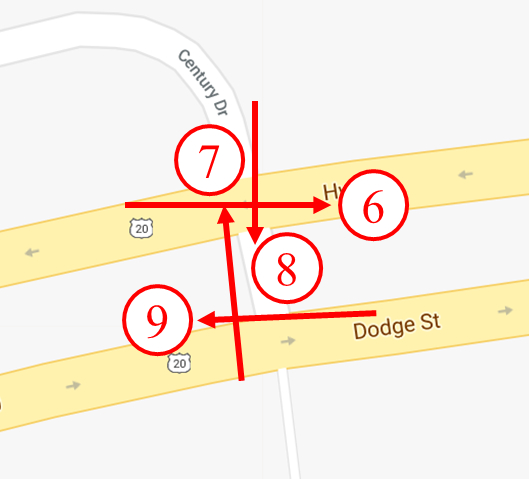
\includegraphics[width=0.7\textwidth]{images/AICityS02.jpg}
    \caption[Topology of an AICity 2022 validation scenario]{Topology of the S02 validation scenario in AICity 2022 Track 1 Dataset}
    \label{fig:AICityS02}
\end{figure}

\begin{table}[ht]
    \centering
    \caption{AICity Challenge 2022 - Track 1 - Details}
    \begin{tabular}{|l|l|l|l|}
    \hline
    \textbf{Camera} & \textbf{Vehicles} & \textbf{Duration} & \textbf{Coordinates}\\ \hline
    \hline
    c006 & 124 & 3m31s & 42.492022, -90.723366 \\ \hline
    c007 & 90 & 3m16s & 42.492109, -90.723946 \\ \hline
    c008 & 99 & 3m12s & 42.491931, -90.723656 \\ \hline
    c009 & 137 & 3m31s & 42.491867, -90.723967 \\ \hline
    \end{tabular}
    \label{table:AICity}
\end{table}

\subsection{Synthetic and Unused Dataset}

\subsubsection{GTA V}
The Multi-Camera Grand Theft Auto (\textbf{MC-GTA}) \cite{MC-GTA} dataset is a synthetic Vehicle Re-Identification benchmark, created using the video game Grand Theft Auto V, from Rockstar Games. The contribution of this dataset addresses several challenges in the development of MTMC systems, where real-world applicability is limited due to the availability of synthetic data. Synthetic datasets, such as MC-GTA, are a practical solution for training robust Computer Vision and Deep Learning-based methods. This avoids the huge human effort required for manual annotation, besides avoiding privacy concerns inherent in real-world datasets.

Annotations for the MC-GTA dataset are collected in an automated manner by interacting with the game engine: vehicles are localized by bounding boxes, and each vehicle is assigned with a unique ID, consistently across all cameras for a specific scenario. It contains \textbf{70} unique vehicles, observed by \textbf{6} cameras placed at three intersections.

The ScriptHookV library was utilized to generate the dataset by allowing interactions with the game engine to extract relevant information. The algorithm for collecting and annotating vehicles iteratively asks the game's engine about the visible vehicles in the view of a network of cameras at any given time. Because GTA-V is a single-player game and does not support native multi-camera synchronization, frames were recorded sequentially by adjusting the position and angle of cameras between captures.

Specifically, the vehicles are filtered on maximum vehicle-to-camera distance, visibility within the camera view, excluding occluded vehicles and vehicles whose engines are off (since they cannot physically transit to another camera). The annotations in the final dataset provide detailed metadata about each collected frame. The structure and content of the annotations are summarized in Table \ref{table:mcgta_annotations}, which also make it suitable for MTMC metrics. Lastly, Camera informations (Position, Rotation and FOVs) are also available. 

\begin{table}[ht]
    \centering
    \caption{MC-GTA Dataset Annotation Format}
    \begin{tabular}{|l|p{10cm}|}
    \hline
    \textbf{Metadata}        & \textbf{Description}                                              \\ \hline
    \textbf{Timestamp}       & Time information about the current frame.                         \\ \hline
    \textbf{FrameID}         & Index of the frame to establish temporal order.                   \\ \hline
    \textbf{LicensePlate}    & Unique license plate identifier for the vehicle.                  \\ \hline
    \textbf{Center(x, y)}    & Coordinates of the vehicle's 2D bounding box center.              \\ \hline
    \textbf{Width}           & Width of the vehicle's 2D bounding box.                           \\ \hline
    \textbf{Height}          & Height of the vehicle's 2D bounding box.                          \\ \hline
    \textbf{Vehicle(x, y, z)} & Coordinates of the vehicle's 3D bounding box.                    \\ \hline
    \end{tabular}
    \label{table:mcgta_annotations}
\end{table}

The MC-GTA dataset has not been widely utilized so far due to technical limitations intrinsic in the GTA V game engine. More specifically, there are lighting inconsistencies across consecutive frames, considering that at timestamp $t$, a vehicle can be in shadow while at $t+1$, it could be under direct sunlight. These sudden changes in lighting conditions can have a negative impact on the performance of vehicle re-identification models, which have to identify the same vehicle under very different lighting conditions within one frame interval.

Also, noise is present, since the HUD of the game is visible in the bottom-left corner of the frame. These shortcomings have been handled in my customized version of this Dataset, by editing the location of intersections and fixing environmental conditions. Although such an approach seemed to be working fine, it introduced another issue which was not present in the original Dataset. Namely, fast rendering between consecutive frames is a very demanding task for a game engine; Because of that, vehicles sometimes spawn suddenly in the middle of a scene. This behavior is a consequence of the internal script that makes the player teleport to every camera position, take a screenshot, and then move on to the next camera.

For the aforementioned difficulties, the MC-GTA dataset was not considered for experiments. However, the material provided is very much worthwhile for further research and future works, assuming subsequent editions refine the methodology and its technical execution.

\subsubsection{VRIC}
The Vehicle Re-Identification in Context (\textbf{VRIC}) \cite{VRIC, VRIC2} dataset was created to address the shortcomings of existing Re-ID benchmarks, which are usually based on synthetic test environments and assume consistent image quality, resolution, and appearance scale. Different from VeRi-776 and similar datasets that mainly focus on high-resolution images with detailed information, VRIC offers a more realistic and challenging benchmark, truthfully reflecting conditions in real-world surveillance applications.

The VRIC dataset includes large variations in image quality and resolution, resulting from uncontrolled variables on the vehicles, such as different image scales, blur caused by motion, changes in illumination, occlusions, and different points of view. All these challenges make VRIC a very good benchmark in testing the robustness of vehicle re-identification methods under unfavorable conditions.

The dataset is created from the UA-Detrac \cite{DETRAC} detection and tracking benchmark by extracting and processing vehicle imagery captured in different road traffic scenarios. The dataset includes a total of \textbf{60,430} images for \textbf{5,622} unique vehicle identities that were taken by 60 cameras under both daytime and nighttime conditions.

This dataset is divided into training and testing sets as described below:
\begin{itemize}
    \item \textit{Training Set}: 2,811 identities with 54,808 images.
    \item \textit{Testing Set}: 2,811 identities with 5,622 images.
\end{itemize}

The following Dataset has been implemented, but not tested, throughout the experiments due to its similarity with the VRU Dataset, but it is still worth mentioning for future research purposes.

\subsection{Metrics}
\subsubsection{Feature Extraction}
In terms of metrics, the Feature Extraction task is evaluated by using standard and common Person Re-Identification evaluation protocols, as in \cite{PersonReID}. Those metrics, which are \textbf{Cumulative Matching Characteristics} (CMC) and \textbf{Mean Average Precision} (mAP), are widely used in academic literature to evaluate the effectiveness of Re-ID models, as they provide a complete understanding of the model's ability to correctly match identities (which could be vehicles, persons, objects, etc.) across different views.

\subsubsection{CMC}
The \textbf{CMC curve} measures recognition under the shape of a ranking problem. It estimates the probability that the correct match is within the top-$k$ elements of a ranked list and is therefore well suited to single-shot recognition problems, such as Vehicle Re-Identification in a single-camera setting.
Formally, let $D$ be the test set of $N$ samples, and rank$_{i}$ be the rank position of the correct match for query$_{i}$. The CMC curve is defined as:
\[
    \text{CMC}(k) = \frac{1}{|\mathcal{D}|} \sum_{i=1}^{|\mathcal{D}|} 1 \cdot \delta_{i},
\]

where:
\begin{itemize}
    \item $\mathcal{D}$ denotes the size of the Test Set,
    \item $\delta_{i}$ is the indicator function that takes value 1 if $\text{query}_i$ is a correct match at $\text{rank}_i \leq k $, 0 otherwise.
\end{itemize}

The CMC curve is more or less like the Receiver Operating Characteristic (ROC) curve, familiar in problems of detections, since it does provide full information about the system with respect to effectiveness of ranking at different thresholds. Higher CMC at lower ranks, say $k = 5$ or $k = 10$, means better performance. The ranks at which the CMC curve will be evaluated are \textit{1, 5, 10}.

\subsubsection{mAP}
The \textbf{Mean Average Precision (mAP)} metric is a measure of recognition in the context of a retrieval task. It measures the average precision of the results retrieved for all the query samples, therefore indicating the model's ability in ranking true positives while penalizing false positives. This particular metric is especially meaningful in multi-shot scenarios where multiple correct matches might exist.

For each vehicle in the Query Set, the goal is to retrieve the same identical vehicle from the Gallery Set. $AP(q)$ for a query image $q$ is defined as:
\[
    AP(q) = \frac{\sum\limits_{k} P(k) \times \delta_{k}}{N_{gt}(q)}
\]

where:
\begin{itemize}
    \item $P(k)$ is the precision at rank $k$,
    \item $\delta_{k}$ is the indicator function that returns 1 if the $k$-th retrieved sample is a true match at rank $\leq k$, 0 otherwise,
    \item $N_{gt}(q)$ is the number of ground truth correspondences for the query $q$.
\end{itemize}

The mAP is then calculated as the average of $AP(q)$ over all the query samples:
\[
    mAP = \frac{1}{|\mathcal{Q}|} \sum_{q=1}^{|\mathcal{Q}|} AP(q)
\]

where $\mathcal{Q}$ denotes the size of the Query Set. A higher mAP indicates better retrieval performance, and a perfect score of 1 means all the relevant matches are retrieved on top of the ranked list.

\subsubsection{MultiTrack Re-Identification}
The performance of MTMC tracking systems is evaluated based on standard metrics, including Identification F1 Score (IDF1), Identification Precision (IDP), Identification Recall (IDR), and Multiple Object Tracking Accuracy (MOTA), as used in \cite{AICityChallenge} and \cite{MTMC-Metrics}. These metrics demonstrate a comprehensive view of how a system can keep identity consistent across different cameras, and it simultaneously quantifies the errors in tracking.

The \textit{IDF1} score balances precision and recall in identity tracking. It is defined as:
\[
\text{IDF1} = \frac{2 \cdot \text{IDTP}}{2 \cdot \text{IDTP} + \text{IDFP} + \text{IDFN}},
\]
where:
\begin{itemize}
    \item \textit{IDTP} is the number of true positive matches for identity assignments,
    \item \textit{IDFP} is the number of false positive identity matches,
    \item \textit{IDFN} is the number of false negatives for identity matches.
\end{itemize}

The \textit{IDP} and \textit{IDR} measure the precision and recall of identities:
\[
\text{IDP} = \frac{\text{IDTP}}{\text{IDTP} + \text{IDFP}}, \quad
\text{IDR} = \frac{\text{IDTP}}{\text{IDTP} + \text{IDFN}}.
\]

The \textit{MOTA} metric measures tracking accuracy by penalizing detection and identity errors:
\[
\text{MOTA} = 1 - \frac{\text{FN} + \text{FP} + \text{IDs}}{\text{GT}},
\]
where:
\begin{itemize}
    \item \textit{FN} is the number of false negatives (missed detections),
    \item \textit{FP} is the number of false positives (spurious detections),
    \item \textit{IDs} is the number of identity switches (track switches),
    \item \textit{GT} is the total number of ground truth tracks.
\end{itemize}

Besides those indicators, other metrics like \textbf{Mostly Tracked (MT)}, \textbf{Partially Tracked (PT)}, and \textbf{Mostly Lost (ML)} gives more extensive information when analyzing the final trajectory quality:
\begin{itemize}
    \item \text{MT}: Tracks detected in at least $\geq 80\%$ of their total extent.
    \item \text{PT}: Tracks found in $< 80\%$ but $\geq 20\%$ of their total length.
    \item \text{ML}: Tracks included in fewer than $< 20\%$ of their total length.
\end{itemize}

These metrics jointly evaluate almost all aspects of MTMC tracking, from detection reliability to identity preservation across cameras, hence providing a strong framework for the evaluation of tracking system performance.

\subsection{Optimizer \& Scheduler}
As already stated in \ref{subsubsec:WarmupScheduler}, the Optimizer and the Scheduler parameters are of great importance for the training process. The Adam optimizer has been selected, with a starting learning rate $lr = 1.5 \times 10^{-4}$ and a weight decay $\gamma = 5.0 \times 10^{-4}$.

In fact, initially, a warmup strategy is applied over the first 10 epochs, which we will denote as $w$, to gradually increase the learning rate from a minimal value $m$ to the base learning rate $b$, ensuring a smooth start for the optimizer. After the warmup phase, the learning rate undergoes a decay schedule until the end of the training process. In addition to the aforementioned decay, the learning rate can also be adjusted at specific epochs using a set of predefined milestones denoted as $s$. The decay factor $\gamma$ is applied at each milestone for most of the decay methods, ensuring controlled step-wise reductions in the learning rate.

Various decay methods have been carried out, as shown in Figure \ref{fig:Schedulers} and these involve using a \textit{Linear}, \textit{Smooth}, \textit{Multi-Step} and \textit{Cosine} decay. Letting $p$ be the power of the cosine decay function, the learning rate $lr(t)$ at epoch $t$ is defined as follows:

\[
    lr(t) = 
    \begin{cases} 
        b & \text{if } t < \text{w} \\
        \max \left( b \cdot 0.5 \cdot \left( 1 + \cos \left( \pi \cdot \left( \frac{t - \text{w}}{T_{\max}} \right)^{p} \right) \right), m \right) & \text{if } \text{w} \leq t < \text{s}[-1] \\
        m & \text{if } t \geq \text{s}[-1]
    \end{cases}
\]

where:
\begin{itemize}
    \item \text{w} = 10
    \item \text{s} = [20, 30, 45, 60, 75, 90, 105, 120, 135, 140]
    \item \text{p} = 1.00
    \item $\text{m} = 1.0 \times 10^{-6}$
    \item $T_{max} = s[-1] - w$
\end{itemize}

The scheduler gradually lowers the learning rate to a minimum value $m$ following the milestones $s$ and the decay given by  the cosine function, ensuring that the model converges to a stable solution.

% Schedulers Figure
\begin{figure}[H]
    \centering
    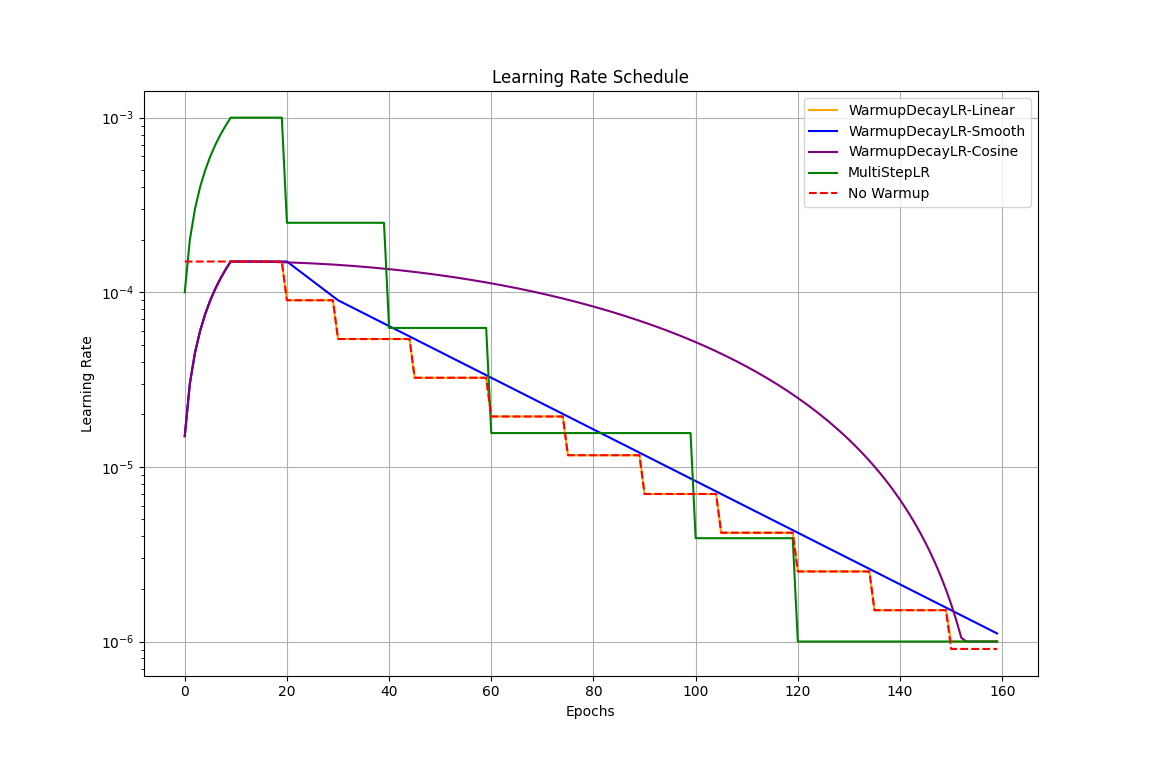
\includegraphics[width=0.90\textwidth]{Images/Schedulers.png}
    \caption[Learning Rate Schedulers]{Different learning rate decay strategies. No-warmup strategy (dotted red line) is also shown.}
    \label{fig:Schedulers}
\end{figure}

\subsection{Data Augmentation}
As for the various data augmentation strategies, the following transformations have been applied to the input images:
\begin{table}[h!]
    \centering
    \begin{tabular}{|l|c|}
        \hline
        \textbf{Name} & \textbf{Value} \\ \hline
        Resize & 320 \\ \hline
        Random Crop (padding) & $p = 0$ \\ \hline
        Random Horizontal Flip (probability) & $p = 0.5$ \\ \hline
        Jitter Brightness (probability) & $p = 0.1$ \\ \hline
        Jitter Contrast (probability) & $p = 0.1$ \\ \hline
        Jitter Saturation (probability) & $p = 0.1$ \\ \hline
        Jitter Hue (probability) & $p = 0.1$ \\ \hline
        Color Augmentation & True \\ \hline
        Padding & 10 \\ \hline
        Random Erasing (probability) & $p = 0.5$ \\ \hline
    \end{tabular}
    \caption{Data augmentation techniques and their values}
    \label{tab:augmentation}
\end{table}

Random cropping has been de-activated due to the fact that cropping the image would result in a squared image, which would not be suitable for the training process. The padding value has been set to 10, to ensure that the image is not cropped and that the aspect ratio is maintained. The Random Erasing technique has been applied with a probability of 0.5, to randomly erase a portion of the image, thus forcing the model to learn more robust features. The Jitter techniques have been applied with a probability of 0.1, to randomly change the brightness, contrast, saturation, and hue of the image, without being too strict on the transformation.

\subsection{MTMC hyperparameters}
\label{subsec:MTMCHyperparameters}

As for the MTMC hyperparameters, there are several parameters that need to be set in order to ensure a smooth tracking process. The following table shows the most important parameters and their values:

\begin{table}[H]
    \centering
    \begin{tabularx}{\textwidth}{l>{\centering\arraybackslash}X}
        \toprule
        \textbf{Parameter} & \textbf{Value} \\ 
        \midrule
        \textbf{YOLO Tracked Classes} & [car, bus, truck, bicycle, motorcycle, train] \\ 
        \textbf{YOLO Confidence Threshold} & 0.20 \\ 
        \textbf{YOLO IOU Threshold} & 0.85 \\
        \textbf{YOLO Image Size} & (640, 640) \\
        \textbf{YOLO Use Agnostic NMS} & True \\
        \textbf{MTMC Similarity Threshold \(\theta_{\text{sim}}\)} & 0.50 \\
        \textbf{MTMC Minimum IOU Threshold} & 0.30 \\
        \textbf{MTMC Drop Single Camera Tracklets} & True \\
        \textbf{Stationary Filtering Minimum Frames $M$} & 1000 \\
        \textbf{Stationary Filtering Threshold $\tau$} & 0.01 \\
        \textbf{Minimum Bounding Box Size $s_{min}$} & 60 \\
        \bottomrule
    \end{tabularx}
    \caption{MTMC Hyperparameters}
    \label{tab:MTMCHyperparameters}
\end{table}

\section{Results}
\subsection{Color Classification}
Initially, a standard SOTA model called \textit{Spectrico} \cite{Spectrico} has been used, which features an extraction, a pre-processing and a classification of the color from the image itself using a MobileNetV3 architecture. The problem lied in the fact that the model was not trained on CCTV images and was not able to generalize well across different scenarios, being also limited to 10 colors only, while VeRi-Wild is composed of 18 colors. For this reason, a custom model has been developed, as stated in \ref{subsubsec:ColorFiltering}. If we take into consideration the Spectrico Model, it performs very bad on the Test Set of \textit{Veri-776} and \textit{VeRi-Wild}, with an accuracy of 43.19\% and 57.09\%, respectively. This is due to the missing color classes, confusing colors such as Yellow with Golden, or Purple with Red, as shown in the Confusion Matrix in Figure \ref{fig:ConfusionMatrixSpectrico}. As shown in Table \ref{tab:ColorClassification}, the custom EfficientNet-B5 model performs much better, with an accuracy of \textbf{91.77\%} and \textbf{94.82\%} on the Test Set of \textit{Veri-776} and \textit{VeRi-Wild}. The confusion matrix in Figure \ref{fig:ConfusionMatrixEfficientNet} shows that the model is able to correctly classify the colors, with a few exceptions, such as the confusion between the colors Orange and Red, or the colors Brown with Golden.

\begin{table}[H]
    \centering
    \begin{tabularx}{\textwidth}{l>{\centering\arraybackslash}X>{\centering\arraybackslash}X>{\centering\arraybackslash}X>{\centering\arraybackslash}X>{\centering\arraybackslash}X}
        \toprule
        \textbf{Model} & \textbf{Dataset Size} & \textbf{Train Loss} & \textbf{Train Accuracy} & \textbf{VeRi-776 Test Accuracy} & \textbf{VeRi-Wild Test Accuracy} \\ 
        \midrule
        Spectrico & - & - & - & 43.19\% & 57.09\% \\ 
        EfficientNet-B3 & 50\% & 0.2941 & 91.77\% & 85.70\% & 91.96\% \\
        EfficientNet-B3 & 100\% & 0.2353 & 93.87\% & 90.66\% & 93.40\% \\ 
        EfficientNet-B5 & 100\% & \textbf{0.2239} & \textbf{94.09\%} & \textbf{91.77\%} & \textbf{94.82\%} \\ 
        \bottomrule
    \end{tabularx}
    \caption{Color Classification Model Accuracy}
    \label{tab:ColorClassification}
\end{table}

\begin{center}
    \begin{figure}[H]
        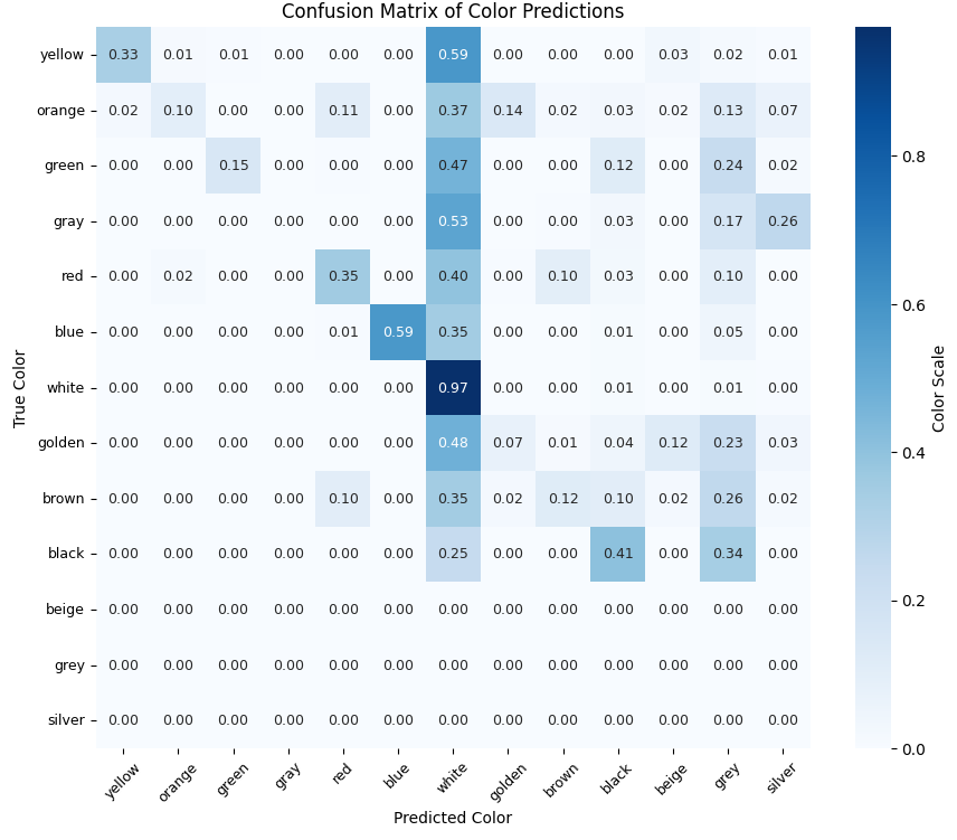
\includegraphics[width=1.00\textwidth]{Images/ConfusionMatrixSpectrico.png}
        \caption[Color Classification Model Accuracy - Spectrico]{Spectrico Model Accuracy on the Test Set of \textit{Veri-776} and \textit{VeRi-Wild}.}
        \label{fig:ConfusionMatrixSpectrico}
    \end{figure}
\end{center}

\begin{center}
    \begin{figure}[H]
        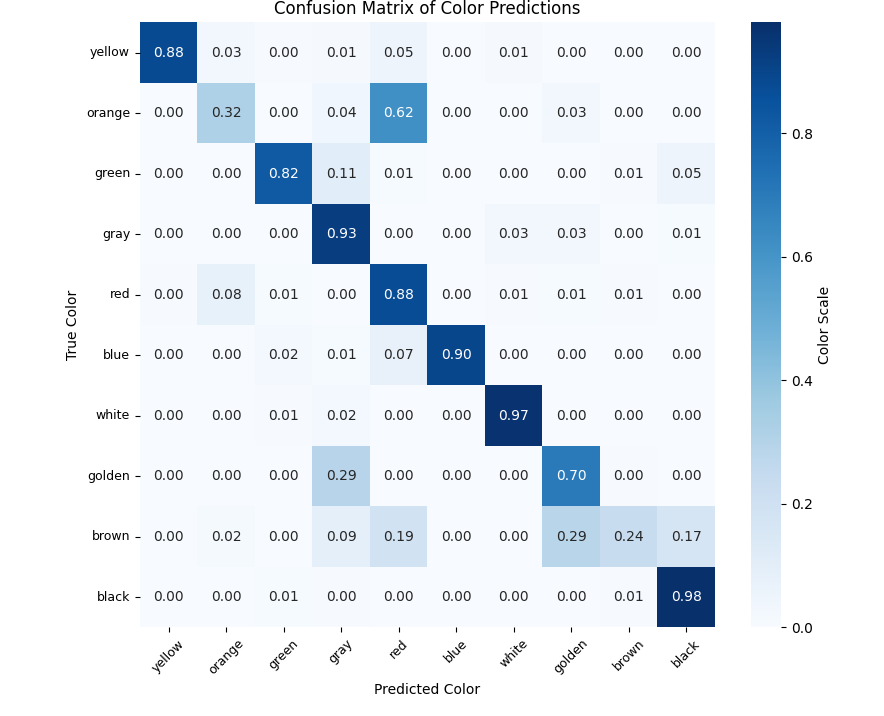
\includegraphics[width=1.00\textwidth]{Images/ConfusionMatrixEfficientNet.png}
        \caption[Color Classification Model Accuracy - EfficientNet]{Color Classification Model Accuracy of the EfficientNet-B5 Model on the Test Set of \textit{VeRi-776}.}
        \label{fig:ConfusionMatrixEfficientNet}
    \end{figure}
\end{center}

\subsection{Re-ID Performance}
In the following subsection, we present the results of training a ReID model for a proper Feature Extraction process. The results presented in Table \ref{tab:ReIDPerformance} provide valuable insights into the impact of different architectural configurations and training strategies on the ReID task, in fact the do present the different configurations and hyperparameters used for the training process, along with the results obtained on the Test Set of the \textit{VeRi-776} Dataset.

\newpage

% NORMAL TABLE BUT NEEDS ID LABELS FOR ANOTHER TABLE
\begin{table}
    \centering % used for centering table
    \resizebox{\columnwidth}{!}{
        \begin{tabular}{|c|c|c|c|c|c|c|c|c|c|c|}
            \hline
            \textbf{ID} & \textbf{Model} & \textbf{GeM} & \textbf{Stride} & \textbf{BNNeck} & \textbf{L. Smooth} & \textbf{MALW} & \textbf{Sampler} & \textbf{Scheduler} & \textbf{Loss} & \textbf{Margin} \\
            \midrule
            1 & ResNet-50 (Baseline) & False & False & False & - & False & None & Linear & Triplet & 1.00 \\ % Test-2
            \hline
            2 & ResNet-50-IBN-a (Baseline) & False & False & False & - & False & None & Linear & Triplet & 1.00 \\ % Test-40
            \hline
            \textcolor{red}{\textit{\textbf{3}}} & ResNet-50-IBN-a & False & True & True & - & False & Random & Warmup Cosine & Triplet & 0.30 \\ % Test-35
            \hline
        \end{tabular}
    }
    
    \vspace{5mm}
    
    \begin{tabular}{|c|c|c|c|c|}
        \hline
        \textbf{ID} & \textbf{mAP} & \textbf{Rank@1} & \textbf{Rank@5} & \textbf{Rank@10}\\ 
        \midrule
        1 & 52.00\% & 72.47\% & 80.87\% & 83.91\% \\ % Test-2
        \hline
        2 & 54.72\% & 75.64\% & 81.21\% & 84.48\% \\ % Test-40
        \hline
        \textcolor{red}{\textit{\textbf{3}}} & \textbf{81.33\%} & \textbf{94.70\%} & \textbf{96.72\%} & \textbf{97.50\%} \\ % Test-35
        \hline
    \end{tabular}
    \vspace{0.5cm}
    \caption[ReID Results]{Results of the ReID model on the \textit{VeRi-776} Test Dataset.}
    \label{tab:ReIDPerformance}
\end{table}

The baseline model, denoted by $ID = 1$, is a standard ResNet-50 without additional modifications or optimizations. With its simplicity, the baseline achieves a mAP of 52.00\%, with Rank@1 and Rank@5 accuracies of 72.47\% and 80.87\%, respectively. These results serve as a reference point for evaluating subsequent improvements.

In contrast, the performance achieved by $ID = 3$, which incorporates various optimizations such as BNNeck, stride adjustment, a cosine scheduler and a Random Dataset Sampler, demonstrates significant gains over the baseline. Specifically, $ID = 3$ achieves an mAP of \textbf{81.33\%}—a substantial increase of over 26 percentage points. Additionally, the Rank@1 accuracy improves to 94.70\%, which serves as an outstanding improvement. This indicates that the modifications applied in $ID = 3$ not only enhance overall retrieval performance but also improve the model's ability to identify the correct vehicle on the first attempt.

Interestingly, $ID = 2$ uses a slightly modified version of the baseline by incorporating the ResNet-50-IBN-a variant, surpassing it by more than 2 points, indicating that IBN could be beneficial in the overall process and improve the model's discriminative power in this specific task.

A closer examination of $ID = 3$ reveals that the combination of BNNeck, a cosine scheduler and the Random Sampler likely contributed to its superior performance. BNNeck, by normalizing feature embeddings, facilitates better generalization and distance-based retrieval, the cosine scheduler aids in more effective learning by gradually reducing the learning rate during training while the Random Sampler ensures a diverse and balanced training dataset.

Overall, these findings highlight the importance of architectural optimizations and training strategies in ReID tasks. While the baseline model provides a solid starting point, advanced configurations such as those used in $ID = 3$ are crucial for achieving state-of-the-art performance. Future work could explore additional improvements, such as incorporating GeM pooling or applying more advanced loss functions to further enhance retrieval accuracy.

\subsection{MTMC Performance}
As for the MTMC performance, a comparison between the main 3 different YOLO architectures is provided by using a ReID model trained on the \textit{AICity} dataset. The results presented in Table \ref{tab:MTMCPerformance} provide insights into the impact of the various hyperparamters explicited in \ref{subsec:Filtering}, \ref{subsec:Unification}, \ref{subsec:MTMC} and \ref{subsec:MTMCHyperparameters} on the MTMC tracking task, highlighting key performance trends and trade-offs. By carefully analyzing the experimental data, several critical insights can be drawn regarding model selection, linkage methods, and tracker performance. Also, a practical and visive result can be appreciated in Figure \ref{fig:MTMCRetrieval}, which shows the retrieval results of the best configuration, $ID = 1$, on the \textit{AICity} dataset for a random set of queries.

% For full experiments table
\begin{sidewaystable}
    \centering
    \resizebox{\textwidth}{!}{ % Resize to fit within page width
        \begin{tabular}{|c|c|c|c|c|c|c|c|c|c|c|c|c|c|c|c|c|c|c|c|c|}
            \hline
            \textbf{ID} & \textbf{YOLO} & \textbf{Tracker} & \textbf{Filters} & \textbf{Confidence}
            & \textbf{Image Size} & \makecell{\textbf{Delete Minimum}\\ \textbf{Frames}} & \textbf{Unification}
            & \makecell{\textbf{Unification}\\ \textbf{Method}}
            & \makecell{\textbf{Similarity}\\ \textbf{Method}}
            & \makecell{\textbf{Linkage}\\ \textbf{Method}}
            & \makecell{\textbf{Similarity}\\ \textbf{Threshold}}
            & \textbf{IDF1} & \textbf{GT} & \textbf{MT} & \textbf{PT}
            & \textbf{ML} & \textbf{IDs} & \textbf{FM} & \textbf{MOTA} \\
            \hline
            \textcolor{red}{\textit{\textbf{1}}} & YoloV11x & \multirow{3}{*}{Custom} & \multirow{3}{*}{False} & 0.20 & (640, 640) & \multirow{3}{*}{True} & \multirow{3}{*}{True} & \multirow{3}{*}{Area Avg} & \multirow{3}{*}{Area Avg}  & \multirow{3}{*}{Mean Feature} & \multirow{3}{*}{0.50} & \textbf{85.0} & 145 & 140 & 5 & 0 & 360 & 561 & \textbf{95.6} \\ % Exp-3 
            2 & YoloV10x & & & 0.20 & (640, 640) & & & & & & & 80.6 & 145 & 139 & 6 & 0 & 390 & 703 & 94.8 \\ % Exp-14
            3 & YoloV9e & & & 0.20 & (640, 640) & & & & & & & 82.8 & 145 & 141 & 4 & 0 & 344 & 684 & 95.1 \\ % Exp-15
            \hline
            \multicolumn{20}{c}{\rule{0pt}{4pt}} \\ % Adds vertical space
            \hline
            4 & YoloV11x & \multirow{11}{*}{Custom} & \multirow{11}{*}{False} & 0.20 & (640, 640) & True & True & Mean & Mean & Mean Feature & \multirow{11}{*}{0.50} & 79.2 & 145 & 139 & 6 & 0 & 385 & 780 & 94.4 \\ % Exp-1 
            5 & YoloV11x & & & 0.20 & (640, 640) & True & True & Area Avg & Mean & Mean Feature & & 79.2 & 145 & 139 & 6 & 0 & 385 & 780 & 94.4 \\ % Exp-4
            6 & YoloV11x & & & 0.20 & (640, 640) & True & True & Area Avg & Area Avg & Average & & 83.9 & 145 & 140 & 5 & 0 & 360 & 563 & 95.6 \\ % Exp-5
            7 & YoloV11x & & & 0.20 & (640, 640) & True & True & Area Avg & Area Avg & Single & & 84.0 & 145 & 140 & 5 & 0 & 360 & 655 & 95.2 \\ % Exp-6
            8 & YoloV11x & & & 0.20 & (640, 640) & True & True & Area Avg & Area Avg & Complete & & 83.8 & 145 & 140 & 5 & 0 & 360 & 624 & 95.3 \\ % Exp-7
            9 & YoloV11x & & & 0.20 & (640, 640) & False & False & Area Avg & Area Avg & Mean Feature & & 80.5 & 145 & 140 & 5 & 0 & 658 & 730 & 93.4 \\ % Exp-10
            10 & YoloV11x & & & 0.50 & (640, 640) & True & True & Area Avg & Area Avg & Mean Feature & & \textbf{86.8} & 145 & 130 & 15 & 0 & 1904 & 420 & 92.8 \\ % Exp-11
            11 & YoloV11x & & & 0.20 & (1280, 1280) & True & True & Area Avg & Area Avg & Mean Feature & & 75.0 & 145 & 142 & 3 & 0 & 285 & 1279 & 92.5 \\ % Exp-13
            12 & YoloV10x & & & 0.20 & (640, 640) & False & False & Area Avg & Area Avg & Mean Feature & & 78.5 & 145 & 138 & 7 & 0 & 684 & 650 & 93.6 \\ % Exp-19
            13 & YoloV9e & & & 0.20 & (640, 640) & False & False & Area Avg & Area Avg & Mean Feature & & 80.3 & 145 & 141 & 4 & 0 & 642 & 634 & 93.9 \\ % Exp-20
            \hline
            \multicolumn{20}{c}{\rule{0pt}{4pt}} \\ % Adds vertical space
            \hline
            14 & YoloV11x & BOTSort & \multirow{5}{*}{False} & 0.20 & (640, 640) & True & True & \multirow{5}{*}{Area Avg} & \multirow{5}{*}{Area Avg} & \multirow{5}{*}{Mean Feature} & \multirow{5}{*}{0.50} & 84.3 & 145 & 141 & 4 & 0 & 294 & 700 & 95.3 \\ % Exp-8  
            15 & YoloV11x & BOTSort & & 0.20 & (640, 640) & False & False & & & & & 81.8 & 145 & 140 & 5 & 0 & 603 & 681 & 93.9 \\ % Exp-22
            16 & YoloV11x & ByteTrack & & 0.20 & (640, 640) & True & True & & & & & 84.3 & 145 & 133 & 11 & 1 & 852 & 756 & 92.3 \\ % Exp-9
            17 & YoloV11x & ByteTrack & & 0.50 & (640, 640) & True & True & & & & & 85.5 & 145 & 120 & 25 & 0 & 588 & 548 & 90.0 \\ % Exp-12
            18 & YoloV11x & ByteTrack & & 0.20 & (640, 640) & False & False & & & & & 84.3 & 145 & 133 & 11 & 1 & 822 & 763 & 92.4 \\ % Exp-21
            \hline
            \multicolumn{20}{c}{\rule{0pt}{4pt}} \\ % Adds vertical space
            \hline
            19 & YoloV11n & \multirow{3}{*}{Custom} & \multirow{3}{*}{False} & 0.20 & (640, 640) & \multirow{3}{*}{True} & \multirow{3}{*}{True} & \multirow{3}{*}{Area Avg} & \multirow{3}{*}{Area Avg} & \multirow{3}{*}{Mean Feature} & \multirow{3}{*}{0.50} & 68.5 & 145 & 37 & 87 & 21 & 7584 & 80 & 63.7 \\ % Exp-16  
            20 & YoloV10n & & & 0.20 & (640, 640) & & & & & & & 73.5 & 145 & 45 & 89 & 11 & 5615 & 81 & 72.8 \\ % Exp-17
            21 & YoloV9t & & & 0.20 & (640, 640) & & & & & & & 71.3 & 145 & 47 & 82 & 16 & 6315 & 49 & 69.6 \\ % Exp-18
            \hline
            \multicolumn{20}{c}{\rule{0pt}{4pt}} \\ % Adds vertical space
            \hline
            22 & YoloV11x & \multirow{3}{*}{Custom} & \multirow{3}{*}{True} & 0.20 & (640, 640) & \multirow{3}{*}{True} & \multirow{3}{*}{True} & \multirow{3}{*}{Area Avg} & \multirow{3}{*}{Area Avg} & \multirow{3}{*}{Mean Feature} & \multirow{3}{*}{0.50} & 7.8 & 145 & 0 & 6 & 129 & 19976 & 5 & 4.7 \\ % Exp-29  
            23 & YoloV10x & & & 0.20 & (640, 640) & & & & & & & 8.0 & 145 & 0 & 16 & 129 & 19950 & 6 & 4.8 \\ % Exp-30
            24 & YoloV9e & & & 0.20 & (640, 640) & & & & & & & 7.8 & 145 & 0 & 15 & 130 & 19965 & 5 & 4.7 \\ % Exp-31
            \hline
            \multicolumn{20}{c}{\rule{0pt}{4pt}} \\ % Adds vertical space
            \hline
            25 & \multirow{6}{*}{YoloV11x} & \multirow{6}{*}{Custom} & \multirow{6}{*}{False} & \multirow{6}{*}{0.20} & \multirow{6}{*}{(640, 640)} & \multirow{6}{*}{True} & \multirow{6}{*}{True} & \multirow{6}{*}{Area Avg} & \multirow{6}{*}{Area Avg} & \multirow{6}{*}{Mean Feature} & \multirow{6}{*}{0.50} & 57.6 & 145 & 140 & 5 & 0 & 360 & 900 & 94 \\ % Exp-23
            26 & & & & & & & & & & & & 58.0 & 145 & 140 & 5 & 0 & 360 & 1019 & 93.4 \\ % Exp-24
            27 & & & & & & & & & & & & 73.0 & 145 & 118 & 23 & 4 & 2168 & 449 & 87.5 \\ % Exp-25
            28 & & & & & & & & & & & & 82.9 & 145 & 138 & 7 & 0 & 432 & 649 & 94.8 \\ % Exp-27
            29 & & & & & & & & & & & & 79.3 & 145 & 140 & 5 & 0 & 367 & 651 & 95.1 \\ % Exp-28
            30 & & & & & & & & & & & & 74.7 & 145 & 139 & 6 & 0 & 402 & 676 & 94.9 \\ % Exp-32       
            \hline
        \end{tabular}
    } % End of resizebox
    \vspace{0.5cm}
    \caption[MTMC Results]{Results of the MTMC task using a ReID model trained on the \textit{AICity} Dataset. Run 25--30 use the same configs but with a different Re-ID backbone.}
    \label{tab:MTMCPerformance}
\end{sidewaystable}

\begin{center}
    \begin{figure}[H]
        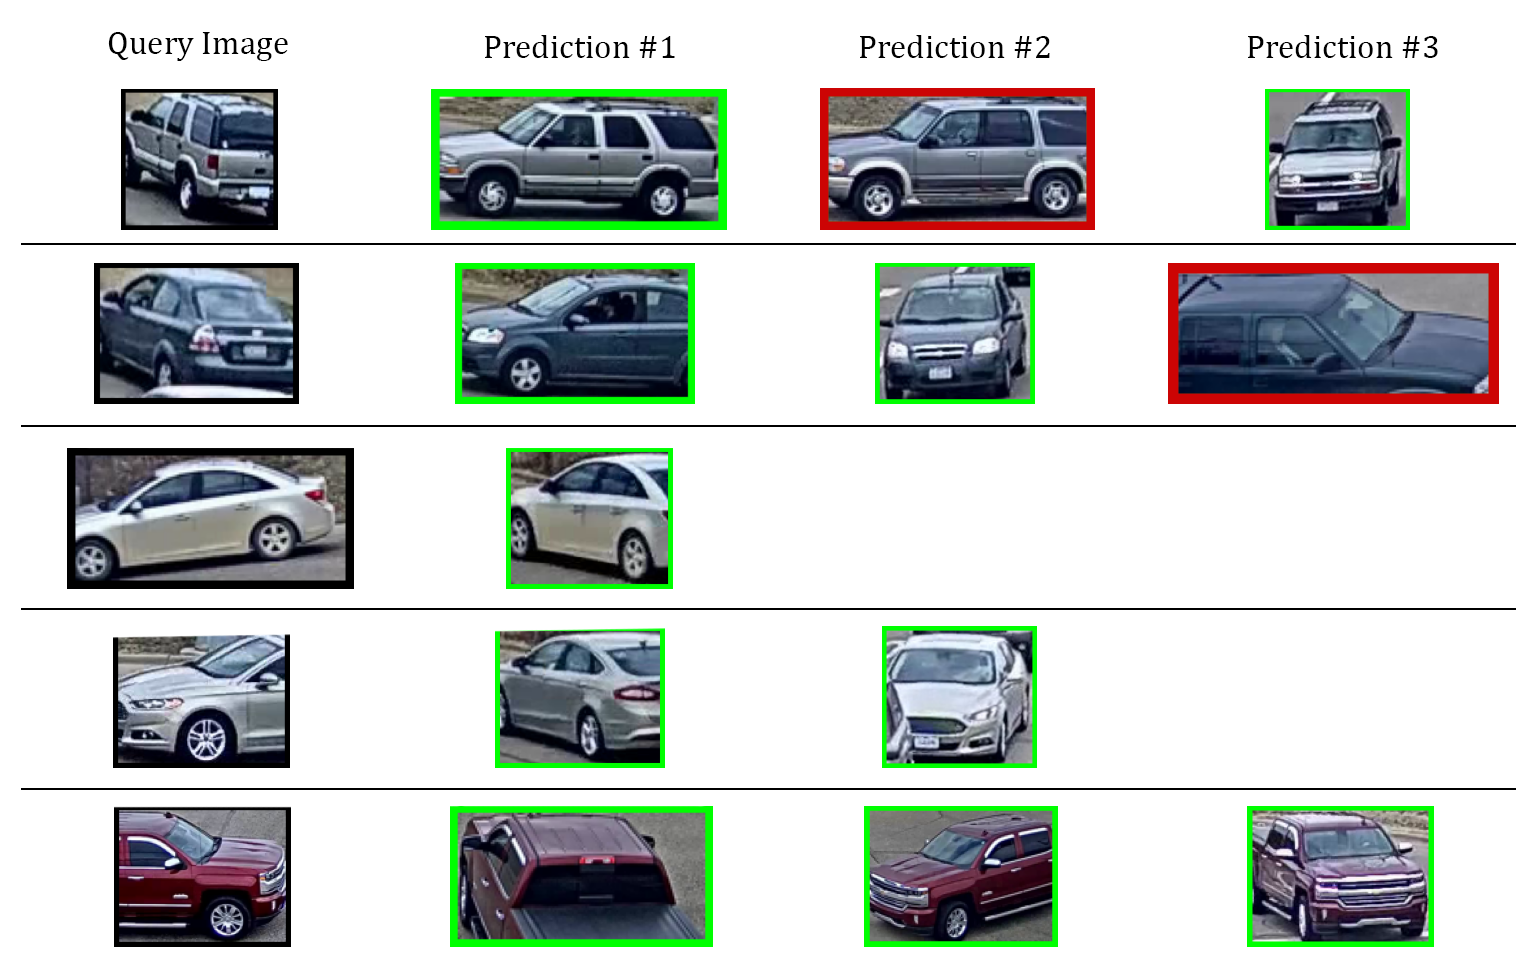
\includegraphics[width=1.00\textwidth]{Images/MTMCRetrieval.png}
        \caption[MTMC Retrieval Results]{MTMC Retrieval Results of the best configuration ($ID = 1$) on the \textit{AICity} dataset.}
        \label{fig:MTMCRetrieval}
    \end{figure}
\end{center}

\subsubsection{YOLO Architecture Comparison}
The first set of experiments (rows 1--3) compares different YOLO architectures: \texttt{YoloV11x}, \texttt{YoloV10x}, and \texttt{YoloV9e}. Despite using the same custom tracker and hyperparameter settings, the results highlight that \texttt{YoloV11x} consistently outperforms the others in terms of IDF1 and MOTA, achieving \textbf{85.0\%} for IDF1 and \textbf{95.6\%} points in the MOTA metric. This suggests that the improved architecture of \texttt{YoloV11x} has a positive impact on MTMC tracking performance.

\subsubsection{Effect of Linkage Methods}
In the subsequent set of experiments (rows 4--8), the focus shifts to evaluating different linkage and unification methods. Specifically, the linkage methods are varied across \texttt{Single}, \texttt{Average}, and \texttt{Complete}. It is evident that different linkage methods (Single, Average, Complete) achieve similar performance levels, with IDF1 scores ranging between 79.2\% and 84.0\%. The Single linkage method slightly edges out others with an IDF1 of 84.0\%, though the differences between Average (83.9\%) and Complete (83.8\%) are minimal, indicating that the MTMC task is relatively robust to linkage method selection within this family of approaches.

\subsubsection{Influence of Different Trackers}
To explore the impact of different tracking algorithms, the experiments in rows 14--18 introduce \texttt{BOTSort} and \texttt{ByteTrack} as alternatives to the custom tracker. Interestingly, while the default \texttt{BOTSort} achieves a competitive MOTA score (95.3\%), the IDF1 score remains slightly lower compared to the custom tracker. This trade-off highlights that the change of some specific hyperparameters could lead to a better performance.

\subsubsection{Degradation of Performance with Model Pruning}
Furthermore, experiments in rows 19--21 demonstrate the performance when using lightweight YOLO versions (\texttt{YoloV11n}, \texttt{YoloV10n}, and \texttt{YoloV9t}). Although these models achieve faster inference times, their IDF1 scores drop significantly (to as low as 68.5\%). This suggests that, for complex tasks such as MTMC, the use of smaller models sacrifices tracking accuracy.

\subsubsection{Impact of Enabling Filtering}
Lastly, rows 22--24 examine the impact of enabling additional filters. As expected, while filtering reduces false positives and improves data cleanliness, it also drastically lowers IDF1 and MOTA scores to below 8.0\% and 5.0\%, respectively. This confirms that excessive filtering can lead to the removal of relevant data, thus harming overall performance.

\section{Ablation Studies}
The following section presents a series of ablation studies conducted to evaluate the impact of individual components on the overall performance of the proposed Re-ID and MTMC system. By systematically analyzing the effects of different configurations and hyperparameters, we aim to identify key factors that contribute to the system's success and provide insights for future improvements.

\subsection{Re-ID Ablation Studies}
The ablation study presented in Table \ref{tab:ReIDAblationStudies} investigates the performance of various configurations across several datasets, including VeRi-776, VeRi-Wild, Vehicle-ID, VRU, and AI-City. The primary objective of this study is to assess the effect of specific components, hyperparameters, and fine-tuning strategies on key evaluation metrics, namely mean Average Precision (mAP), Recall at 1 (R@1), Recall at 5 (R@5), and Recall at 10 (R@10).

% For full experiments table
\begin{sidewaystable}
    \centering
    \resizebox{\textwidth}{!}{ % Resize to fit within page width
    \begin{tabular}{|c|c|c|c|c|c|c|c|c|c|c|c|c|c|c|c|c|}
        \hline
        \textbf{ID} & \textbf{Dataset} & \textbf{Model} & \textbf{GeM} & \textbf{Stride} & \textbf{BNNeck} &
        \textbf{Margin} & \textbf{L. Smoothing} & \textbf{MALW} & \textbf{Scheduler} & \textbf{Sampler} &
        \textbf{Loss} & \textbf{RPTM} & \textbf{mAP} & \textbf{R@1} & \textbf{R@5} & \textbf{R@10} \\
        \hline
        4 & \multirow{19}{*}{VeRi-776} & \multirow{3}{*}{ResNet-50} & False & False & False & \multirow{3}{*}{0.30} & - & False & \multirow{3}{*}{Warmup Linear} & \multirow{3}{*}{Random} & \multirow{3}{*}{Triplet} & \multirow{3}{*}{False} & 66.68\% & 91.66\% & 96.72\% & 97.38\% \\
        5 &  &  & True & True & True & & 0.10 & True & & & & & 70.40\% & 92.67\% & 96.31\% & 98.21\% \\
        6 &  &  & False & True & True & & - & False & & & & & 68.94\% & 92.49\% & 97.20\% & 98.14\% \\
        \cline{3-17}
        7 & \multirow{14}{*}{} & \multirow{14}{*}{ResNet-50-IBN-a} & False & \multirow{14}{*}{True} & True & 1.00 & - & False & Warmup Smooth & Random & Triplet & False & 74.12\% & 95.17\% & 97.79\% & 98.39\% \\
        8 &  &  & False & & True & 1.00 & - & False & Warmup Cosine & Random & Triplet & False & 77.19\% & \textbf{96.42\%} & \textbf{98.39\%} & \textbf{99.40}\% \\
        9 &  &  & False & & True & 1.00 & 0.00173 & True & Warmup Cosine & Random & Triplet & False & 77.80\% & 93.50\% & 95.29\% & 96.25\% \\
        10 &  &  & False & & True & 0.30 & 0.00173 & True & Warmup Cosine & Random & Triplet & False & \textbf{79.14\%} & 95.11\% & 96.60\% & 97.02\% \\
        11 &  &  & True & & True & 0.30 & - & False & Warmup Cosine & Random & Triplet & False & 71.66\% & 93.50\% & 95.11\% & 95.95\% \\
        12 &  &  & True & & True & 1.00 & - & False & Warmup Cosine & Random & Triplet & False & 72.30\% & 93.09\% & 95.35\% & 96.19\% \\
        13 &  &  & False & & True & 0.30 & - & False & Warmup Cosine & Random & MultiSupCon & False & 78.75\% & 93.50\% & 96.01\% & 96.90\% \\
        14 &  &  & True & & True & 1.00 & 0.00173 & True & Warmup Cosine & Random & Triplet & False & 69.35\% & 93.33\% & 95.11\% & 96.19\% \\
        15 &  &  & True & & True & 1.00 & - & True & Warmup Smooth & Random & Triplet & False & 72.26\% & 95.29\% & 97.74\% & 98.57\% \\
        16 &  &  & False & & True & 1.00 & - & False & Warmup MultiStep & None & Triplet & True (Mean) & 71.23\% & 94.93\% & 98.15\% & 98.81\% \\
        17 &  &  & False & & False & 1.00 & - & False & Warmup Smooth & None & Triplet & True (Mean) & 63.56\% & 88.80\% & 96.01\% & 97.44\% \\
        18 &  &  & False & & False & 1.00 & - & False & Warmup MultiStep & None & Triplet & True (Mean) & 67.18\% & 92.25\% & 96.19\% & 98.15\% \\
        19 &  &  & False & & True & 1.00 & - & False & Warmup Linear & None & Triplet & True (Mean) & 67.83\% & 93.33\% & 97.32\% & 98.39\% \\
        \cline{3-17}
        20 &  \multirow{2}{*}{} & \multirow{2}{*}{ResNet-101-IBN-a} & \multirow{2}{*}{False} & \multirow{2}{*}{True} & \multirow{2}{*}{True} & \multirow{2}{*}{1.00} & \multirow{2}{*}{-} & \multirow{2}{*}{False} & Warmup Smooth & \multirow{2}{*}{Random} & \multirow{2}{*}{Triplet} & \multirow{2}{*}{False} & 74.60\% & 95.29\% & 97.85\% & 98.27\% \\
        21 & & & & & & & & & Warmup Cosine & & & & 78.87\% & 96.25\% & 98.57\% & 99.11\% \\
        \hline
        \multicolumn{17}{c}{\rule{0pt}{4pt}} \\ % Adds vertical space
        \hline
        22 & VeRi-Wild (Small) & ResNet-50-IBN-a & False & True & True & 1.00 & - & False & Warmup Cosine & Random & Triplet & False & 76.75\% & 91.03\% & 96.89\% & 98.16\% \\
        \hline
        \multicolumn{17}{c}{\rule{0pt}{4pt}} \\ % Adds vertical space
        \hline
        23 & \multirow{2}{*}{Vehicle-ID (Small)} & ResNet-50-IBN-a & \multirow{2}{*}{False} & \multirow{2}{*}{True} & \multirow{2}{*}{True} & \multirow{2}{*}{1.00} & \multirow{2}{*}{-} & \multirow{2}{*}{False} & \multirow{2}{*}{Warmup Cosine} & \multirow{2}{*}{Random} & \multirow{2}{*}{Triplet} & \multirow{2}{*}{False} & 85.45\% & 79.87\% & 92.41\% & 95.26\% \\
        24 & & ResNet-101-IBN-a & & & & & & & & & & & 86.55\% & 80.91\% & 94.05\% & 96.29\% \\       
        \hline
        \multicolumn{17}{c}{\rule{0pt}{4pt}} \\ % Adds vertical space
        \hline
        25 & VRU (Small) & \multirow{2}{*}{ResNet-50-IBN-a} & \multirow{2}{*}{False} & \multirow{2}{*}{True} & \multirow{2}{*}{True} & \multirow{2}{*}{1.00} & \multirow{2}{*}{-} & \multirow{2}{*}{False} & \multirow{2}{*}{Warmup Smooth} & \multirow{2}{*}{Random} & \multirow{2}{*}{Triplet} & \multirow{2}{*}{False} & 97.48\% & 99.75\% & 100.00\% & 100.00\% \\
        26 & VRU (Medium) & & & & & & & & & & & & 96.10\% & 99.50\% & 99.83\% & 99.87\% \\
        \hline
        \multicolumn{17}{c}{\rule{0pt}{4pt}} \\ % Adds vertical space
        \hline
        27 & \multirow{4}{*}{AI-City} & \multirow{4}{*}{ResNet-50-IBN-a} & \multirow{4}{*}{False} & \multirow{4}{*}{True} & \multirow{4}{*}{True} & \multirow{4}{*}{1.00} & - & False & \multirow{4}{*}{Warmup Cosine} & \multirow{4}{*}{Random} & Triplet & \multirow{4}{*}{False} & - & - & - & - \\
        28 & & & & & & & - & False & & & MultiSupCon & & - & - & - & - \\
        29 & & & & & & & 0.00227 & True & & & Triplet & & - & - & - & - \\
        30* & & & & & & & - & False & & & Triplet & & - & - & - & - \\
        \hline
    \end{tabular}
    } % End of resizebox
    \vspace{0.5cm}
    \caption[ReID Ablation Studies]{Ablation Study for the Re-ID model on different datasets. * denotes a fine-tuned model. The metrics for AI-City are unavailable due to the missing Validation Set.}
    \label{tab:ReIDAblationStudies}
\end{sidewaystable}

\subsubsection{General Trends Across Configurations}
\begin{enumerate}
    \item \textbf{Impact of Model Architecture}:
    \begin{itemize}
        \item The ResNet-50 and ResNet-50-IBN-a models are extensively compared across multiple datasets. The inclusion of Instance Batch Normalization (IBN) layers in ResNet-50-IBN-a provides a noticeable performance boost, in fact, for the VeRi-776 dataset, the run with ID 8 (ResNet-50-IBN-a with Warmup Cosine Scheduler and Triplet loss) achieves a mAP of 77.19\%, outperforming the ResNet-50 model with ID 5, which records a mAP of 70.40\%.
        \item Similarly, the use of ResNet-101-IBN-a in ID 24 for the Vehicle-ID (Small) dataset yields superior results compared to ResNet-50-IBN-a in ID 23, improving mAP from 85.45\% to 86.55\%, indicating that deeper networks can enhance Re-ID performance at the cost of computational complexity.
    \end{itemize}
    
    \item \textbf{Impact of BNNeck}:
    \begin{itemize}
        \item The inclusion of Batch Normalization Neck (BNNeck) demonstrates significant improvements in performance. This is particularly evident when comparing ID 17 (without BNNeck, mAP: 63.56\%) to ID 16 (with BNNeck, mAP: 71.23\%) under otherwise identical configurations (with an exception for the MultiStep scheduler). The positive effect of BNNeck is consistent across different schedulers and loss functions, suggesting its importance in the Re-ID pipeline.
    \end{itemize}
    
    \item \textbf{Scheduler Variations}:
    \begin{itemize}
        \item Warmup Cosine and Warmup Smooth schedulers consistently outperform other scheduling strategies. In the VeRi-776 dataset, switching from a Warmup Linear scheduler (ID 19, mAP: 67.83\%) to a Warmup Cosine scheduler (ID 8, mAP: 77.19\%) with Triplet Loss results in a substantial improvement in performance.
        \item The effectiveness of the Warmup Cosine scheduler is particularly evident in configurations using the ResNet-50-IBN-a architecture, where it consistently achieves higher mAP scores.
    \end{itemize}
\end{enumerate}

\subsubsection{Dataset-Specific Performance}
\begin{enumerate}
    \item \textbf{VeRi-776 Dataset}:
    \begin{itemize}
        \item The best performance in the ablation study is achieved by ID 10 (ResNet-50-IBN-a, Warmup Cosine scheduler, Triplet loss with Margin $\alpha = 0.30$ and MALW), reaching a mAP of 79.14\%. This configuration demonstrates that the combination of appropriate margin values and loss weighting can significantly enhance performance.
        \item Global Average Pooling (GeM) consistently shows reduced performance compared to standard pooling methods. This is evident when comparing ID 11 (with GeM, mAP: 71.66\%) to ID 8 (without GeM, mAP: 77.19\%) under similar configurations. This suggests that GeM may not be well-suited for this specific Re-ID task or it needs a proper tuning.
    \end{itemize}
    
    \item \textbf{VRU Dataset}:
    \begin{itemize}
        \item Exceptional performance is observed on both VRU Small and Medium variants (IDs 25 and 26), with near-perfect recall scores (R@5 and R@10 reaching 100\% for Small, and 99.83\% and 99.87\% for Medium respectively).
        \item The high performance across different dataset sizes suggests the robustness of the chosen architecture and training strategy for this specific Re-ID scenario.
    \end{itemize}
    
    \item \textbf{Vehicle-ID Dataset}:
    \begin{itemize}
        \item ResNet-101-IBN-a (ID 24) demonstrates superior performance over ResNet-50-IBN-a (ID 23), with improvements in all metrics (mAP: 86.55\% vs 85.45\%).
        \item The deeper architecture proves particularly beneficial for this dataset, suggesting that increased model capacity helps capture more discriminative features.
    \end{itemize}
\end{enumerate}

\subsubsection{Key Findings and Insights}
\begin{itemize}
    \item \textbf{Architectural Components}: The combination of IBN-enhanced architectures with BNNeck consistently improves performance across datasets. In particular, ResNet-101-IBN-a provides additional benefits when computational resources permit its use.
    
    \item \textbf{Training Strategy}: The Warmup Cosine scheduler emerges as the most effective learning rate strategy, particularly when combined with appropriate margin values in the Triplet loss (ideally with $\alpha = 0.30$).
    
    \item \textbf{Momentum Adaptive Loss Weight (MALW)}: While MALW shows impressive and really nice results in specific configurations (as in ID 10), its impact varies across different setups. The best mAP score on VeRi-776 (79.14\%) was achieved with MALW enabled, suggesting its potential when properly configured. In other configurations, however, MALW may not always lead to performance improvements, underscoring the need for careful tuning and evaluation in the Re-ID pipeline.
    
    \item \textbf{MultiSupCon Loss}:
    A noteworthy observation from our ablation studies is the performance of MultiSupCon loss (ID 13), which achieves a highly competitive mAP of 78.75\% on the VeRi-776 dataset. This configuration, using ResNet-50-IBN-a with BNNeck and Warmup Cosine scheduler, demonstrates that MultiSupCon loss is a strong alternative to the traditional Triplet loss approach. While it doesn't quite reach the peak performance of our best Triplet loss configuration (ID 3 with 81.33\% mAP), it offers several interesting characteristics since it achieves strong results across all metrics (93.50\% R@1, 96.01\% R@5, 96.90\% R@10). All of this, of course, is enhanced by the fact that unlike Triplet loss which requires careful margin tuning ($\alpha$ parameter), MultiSupCon provides competitive results without this additional hyperparameter.
\end{itemize}

In conclusion, our ablation studies reveal the critical importance of architectural choices (IBN layers, BNNeck) and training strategies (Warmup Cosine scheduling) in Re-ID performance. The varying impact of components like MALW and GeM across different configurations highlights the need for careful consideration of the complete pipeline rather than individual components in isolation. These findings provide valuable direction for future research in vehicle Re-ID systems.

\subsection{MTMC Ablation Studies}
In the MTMC Ablation studies, the main goal is to evaluate the MTMC performances in terms of computational efficiency, resource utilization, and the impact of various system components.
The Table \ref{tab:MTMCAblationStudies} investigates these aspects, which could be summarized as follows:

\begin{sidewaystable}
    \centering
    \resizebox{\textwidth}{!}{ % Resize to fit within page width
        \begin{tabular}{|c||c|c|c|c|c|c|c|c|c|c|c|c|c|c|}
            \hline
            % 13 columns
            \makecell{\textbf{ID from}\\ \textbf{MTMC Table}} & \textbf{N. BBoxes} & \textbf{N. IDs} & \makecell{\textbf{BBoxes}\\ \textbf{Removed}}
            & \makecell{\textbf{Color}\\ \textbf{Removed}} & \makecell{\textbf{Stationary}\\ \textbf{Removed}}
            & \makecell{\textbf{Incomplete}\\ \textbf{Removed}} & \makecell{\textbf{YOLO Detection +}\\ \textbf{Tracking (ms)}}
            & \textbf{Main Filtering (ms)}  & \textbf{Re-ID (ms)} & \makecell{\textbf{Trajectory}\\ \textbf{Creation (ms)}}
            & \textbf{Database (ms)} & \textbf{Unification (ms)} & \textbf{DB Size} & \makecell{\textbf{ID from}\\ \textbf{ReID Table}} \\
            \hline
            1 & 45144 & 535 & - & - & - & - & 40.56 & - & 781.05 & 150.64 & 188.15 & 3798.61 & 2979.19 MB & 27 \\
            2 & 46637 & 543 & - & - & - & - & 40.00 & - & 784.29 & 147.24 & 189.62 & 3194.02 & 3024.66 MB & 27 \\
            3 & 45876 & 551 & - & - & - & - & 46.24 & - & 757.10 & 146.84 & 184.53 & 3887.31 & 2997.48 MB & 27 \\
            \hline
            \multicolumn{13}{c}{\rule{0pt}{2.5pt}} \\ % Adds vertical space
            \hline
            9 & 45210 & 565 & - & - & - & - & 40.53 & - & 748.03 & 146.05 & 183.52 & - & 2998.23 MB & 27 \\
            11 & 68693 & 609 & - & - & - & - & 73.89 & - & 990.68 & 140.54 & 240.83 & 14488.59 & 3720.22 MB & 27 \\
            12 & 46742 & 591 & - & - & - & - & 39.99 & - & 749.03 & 139.24 & 176.88 & - & 3043.64 MB & 27 \\
            13 & 45943 & 582 & - & - & - & - & 46.13 & - & 727.64 & 142.10 & 177.78 & - & 3013.86 MB & 27 \\
            \hline
            \multicolumn{13}{c}{\rule{0pt}{2.5pt}} \\ % Adds vertical space
            \hline
            14 & 47214 & 561 & - & - & - & - & 40.63 & - & 779.37 & 145.44 & 186.17 & 3861.71 & 3067.12 MB & 27 \\
            15 & 47294 & 601 & - & - & - & - & 40.61 & - & 736.66 & 139.44 & 178.80 & - & 3086.98 MB & 27 \\
            16 & 47358 & 551 & - & - & - & - & 15.96 & - & 786.13 & 129.18 & 192.51 & 14369.53 & 2852.23 MB & 27 \\
            17 & 40164 & 563 & - & - & - & - & 15.81 & - & 645.05 & 122.20 & 159.25 & 10419.80 & 2571.91 MB & 27 \\
            18 & 47496 & 607 & - & - & - & - & 16.10 & - & 717.82 & 123.49 & 119.13 & - & 2882.21 MB & 27 \\
            \hline
            \multicolumn{13}{c}{\rule{0pt}{2.5pt}} \\ % Adds vertical space
            \hline
            19 & 21976 & 438 & - & - & - & - & 33.62 & - & 475.14 & 126.45 & 119.04 & 3631.22 & 1748.87 MB & 27 \\
            20 & 22285 & 448 & - & - & - & - & 33.79 & - & 468.18 & 130.74 & 115.96 & - & 1849.06 MB & 27 \\
            21 & 22993 & 429 & - & - & - & - & 37.72 & - & 519.47 & 135.66 & 124.47 & - & 1867.03 MB & 27 \\
            \hline
            \multicolumn{13}{c}{\rule{0pt}{2.5pt}} \\ % Adds vertical space
            \hline
            22 & 4115 & 71 & 40468 & 19973 & 3822 & 16673 & 41.71 & 1226.84 & 650.09 & 119.97 & 94.75 & 1324.39 & 315.96 MB & 27 \\
            23 & 5346 & 77 & 41363 & 19983 & 3947 & 17643 & 40.57 & 1237.15 & 672.02 & 118.48 & 90.28 & 1431.12 & 375.57 MB & 27 \\
            24 & 4687 & 74 & 41215 & 19933 & 2604 & 18678 & 46.15 & 1228.25 & 660.13 & 122.11 & 106.84 & 1412.36 & 347.19 MB & 27 \\
            \hline
            \multicolumn{13}{c}{\rule{0pt}{2.5pt}} \\ % Adds vertical space
            \hline
            25 & 45144 & 535 & - & - & - & - & 40.63 & - & 640.80 & 149.94 & 187.82 & 3699.41 & 2979.19 MB & 1 \\
            26 & 45144 & 534 & - & - & - & - & 40.54 & - & 770.54 & 149.92 & 185.36 & 3684.10 & 2979.19 MB & 2 \\
            27 & 45144 & 535 & - & - & - & - & 40.57 & - & 775.84 & 150.19 & 185.82 & 3758.35 & 2979.19 MB & 8 \\
            28 & 45144 & 535 & - & - & - & - & 40.63 & - & 775.96 & 150.02 & 189.57 & 3743.044 & 2979.19 MB & 30* \\
            29 & 45144 & 535 & - & - & - & - & 40.58 & - & 771.09 & 150.42 & 188.23 & 3843.09 & 2979.19 MB & 28 \\
            30 & 45144 & 535 & - & - & - & - & 41.77 & - & 863.33 & 155.76 & 121.29 & 4127.59 & 2979.19 MB & 29 \\
            \hline
        \end{tabular}
    } % End of resizebox
    \vspace{0.5cm}
    \caption[MTMC Ablation Studies]{Ablation Study for the MTMC task using a ReID model trained on the \textit{AICity} Dataset.}
    \label{tab:MTMCAblationStudies}
\end{sidewaystable}

First, we examined the baseline configurations (Experiments 1-3) using different YOLO architectures (V11x, V10x, and V9e). These experiments demonstrated remarkable consistency in their computational footprint, maintaining database sizes around 3GB and comparable processing times across all pipeline stages.

A particularly intriguing observation emerged when adjusting the detection confidence threshold (Experiment 11). Increasing this parameter to 0.50 led to a substantial rise in detected bounding boxes—approximately 50\% more than the baseline—consequently resulting in significantly longer unification times ($\sim$14.5s versus $\sim$3.8s) and increased memory requirements. Also, even if it increased the overall IDF1 metric with a score (85.5\%), also the number of false positives increased, which is a trade-off that needs to be considered. Actually, the number of PT (Partially Tracked IDs) increased from 5 to 25, leading us to believe that the pipeline is not able to correctly match the detections with the ground truth.

The tracker comparison (Experiments 14-18) yielded noteworthy results. While ByteTrack demonstrated superior efficiency in the detection and tracking times ($\sim$16ms versus $\sim$40ms for other trackers), the overall MTMC performance degradated with respect to the custom tracker due to a lower number of MT (Mostly Tracked IDs) which went from 140, of the Experiment 3, to 133 with also an increase of ID switches.

Perhaps the most significant impact on system performance came from our filtering mechanisms (Experiments 22-24). The implementation of filters resulted in:
\begin{itemize}
    \item A dramatic reduction in processed bounding boxes (from $\sim$45,000 to $\sim$4,000-5,000)
    \item Substantial decrease in database size (down to $\sim$315-375MB from $\sim$3GB)
    \item Additional processing overhead of approximately 1.2 seconds for filtering
\end{itemize}

The implementation of Filtering in Target Mode demonstrates a significant enhancement in system performance compared to the non-filtered pipeline. This improvement manifests in two key aspects: operational efficiency and retrieval accuracy. From an operational perspective, the filtering mechanism substantially reduces both the number of processed bounding boxes and the overall database size, leading to improved computational efficiency. The qualitative analysis presented in Figure \ref{fig:MTMCPerformance} reveals even more compelling results regarding retrieval accuracy. Without filtering, the system only identifies two instances of the Target Vehicle, with subsequent predictions (Top-2 and Top-3) showing significant mismatches, including inappropriate vehicle types (trucks) and incomplete detections. In contrast, the filtered approach demonstrates marked improvements by successfully identifying at least one additional occurrence of the Target Vehicle and the Top-2 and Top-3 predictions exhibit notably higher visual similarity to the Target Vehicle, displaying more consistent vehicle types and complete detections. These improvements in both retrieval accuracy and prediction quality strongly validate the effectiveness of the filtering mechanism in Target Mode operation. The results suggest that filtering not only optimizes system resources but also significantly enhances the quality of vehicle matching and identification, which is a great advantage.

% Include MTMC Performance Figure
\begin{figure}[H]
    \centering
    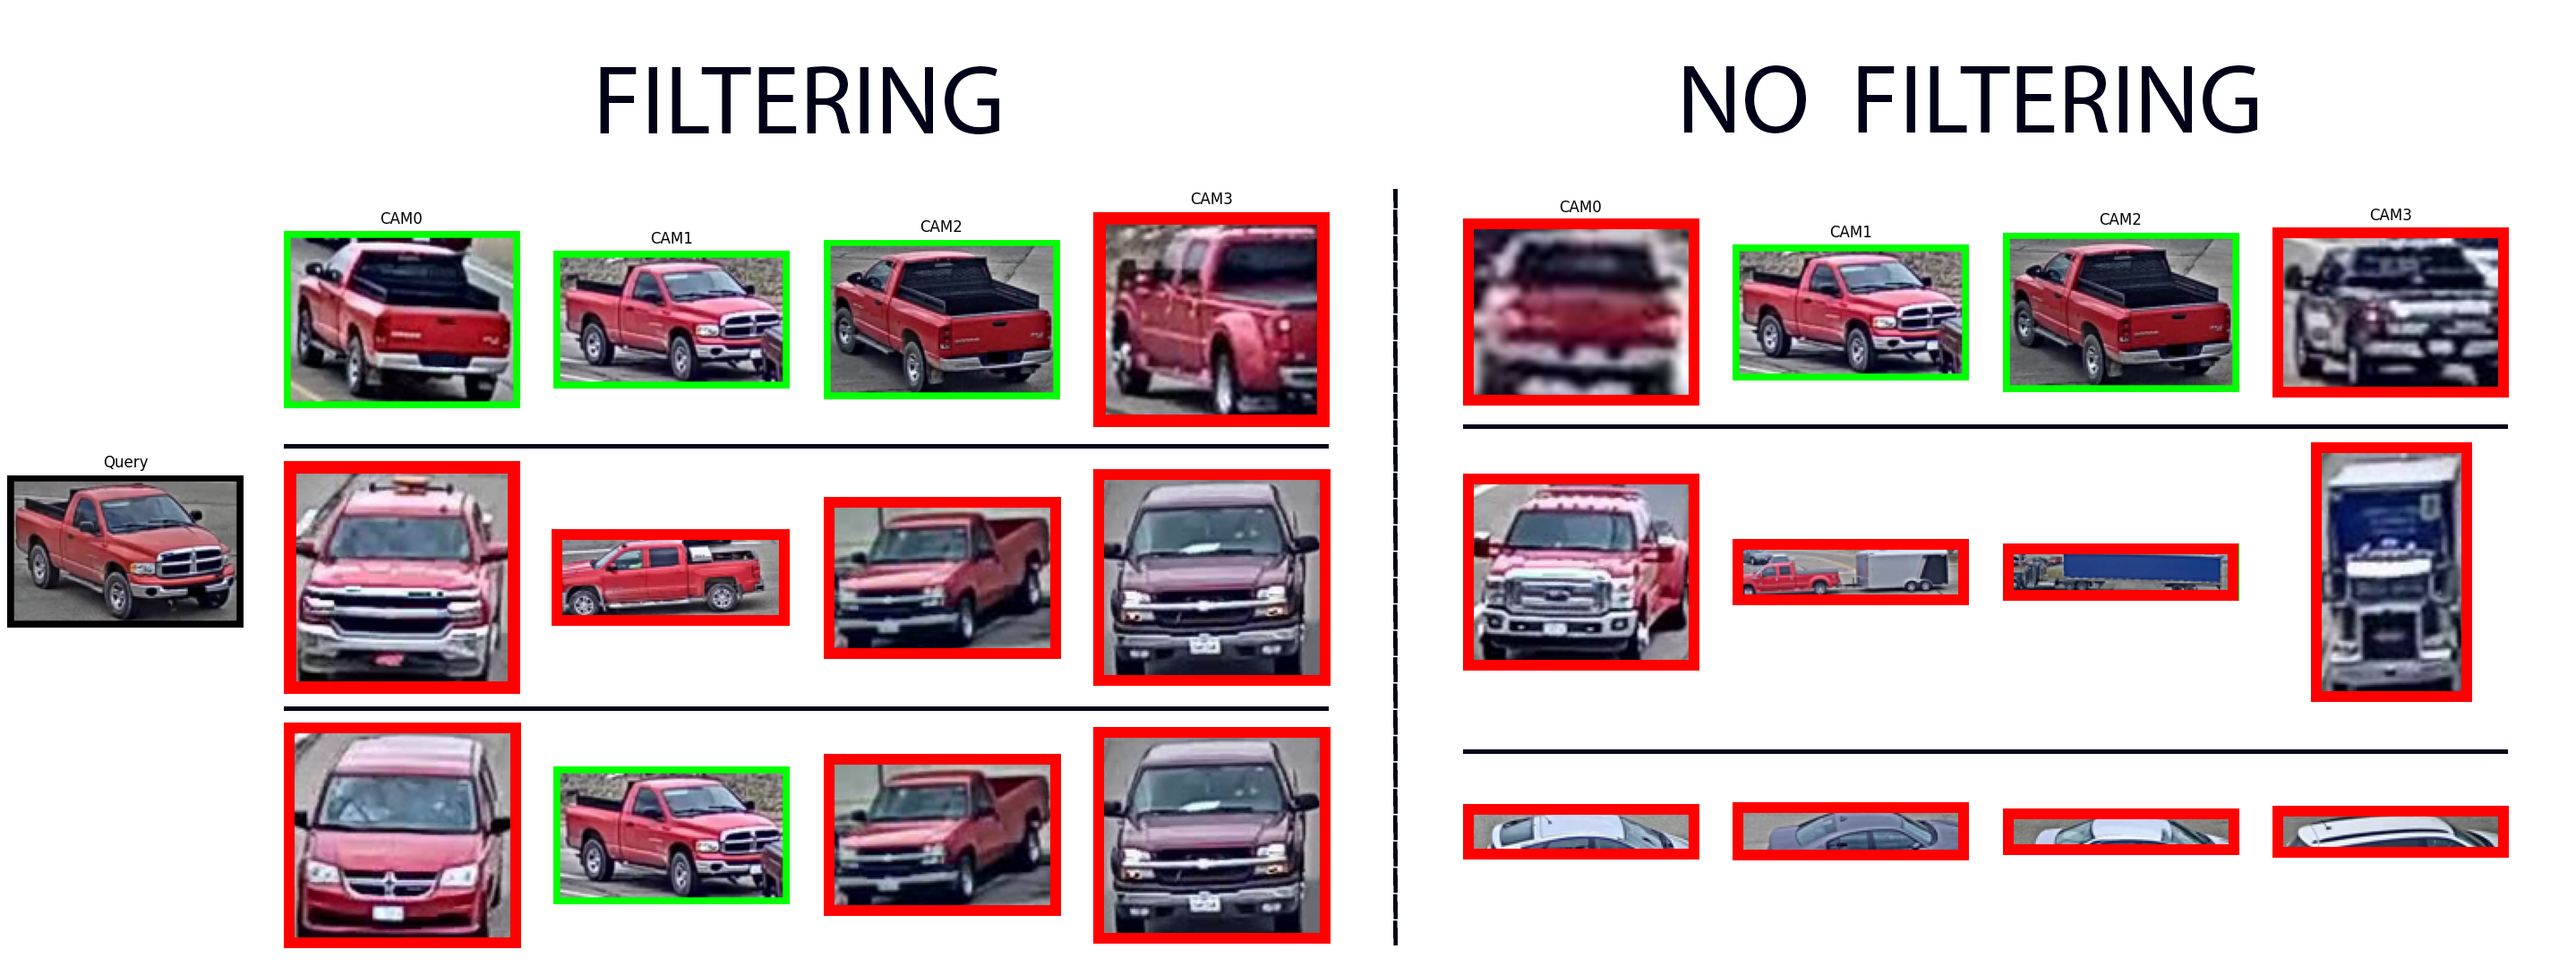
\includegraphics[width=1.0\textwidth]{images/MTMCPerformance.png}
    \caption[MTMC Performance]{Pipeline (\textit{Target Mode}) performance comparison between the baseline and the filtering mechanism. Rows denote the top-k prediction. We can see that Filtering helps in finding at least one other occurence of the Target Vehicle in the database.}
    \label{fig:MTMCPerformance}
\end{figure}

Finally, our investigation of different ReID models (Experiments 25-30) revealed a remarkably stable system behavior, with consistent detection counts and database sizes, suggesting that our pipeline architecture is robust across varying ReID configurations. Specifically, we can infer that Experiment 28 (which used a model trained on VeRi-776 and fine-tuned on AICity) has a lower IDF1 score (82.9) compared to Experiment 1, where a training from stratch on AI-City dataset was used (with an IDF1 score of 85.0). This suggests that the fine-tuning process may not always lead to performance improvements, and that the choice of training a model from stratch on a specific dataset can have a significant impact on the final results.

These findings provide valuable insights for system optimization and deployment considerations, particularly in scenarios where computational resources or real-time processing requirements are critical constraints.
